\documentclass{beamer}
\usetheme{Berlin}
% \usecolortheme{beaver}
%\useoutertheme[subsection=False]{miniframes}
% \useinnertheme{rounded}
% \beamertemplatenavigationsymbolsempty
% \setbeamercovered{transparent=10}
\setbeamercovered{dynamic}
%\usefonttheme{serif}

%\usepackage{beamerthemesplit}
%\usepackage{beamerthemeshadow}
\usepackage{lipsum}  
\usepackage{hyperref}
\usepackage{colortbl}

\title[Beamer]{Beamer Tutorial}
\subtitle{CS 213: Software Systems Laboratory}

\author{Tamal Das}
\institute[CSE, IITDh]{Department of Computer Science and Engineering \\ IIT Dharwad}

% \author[author1 et al.]{author1\inst{1} \and author2\inst{2}}
% \institute[Location1 and Location 2]{
% \inst{1} Affiliation 1 \and
% \inst{2} Affiliation 2}

\date{\today}

% \AtBeginSection[]
% {
%   \begin{frame}
%     \frametitle{Table of Contents}
%     \tableofcontents[currentsection]
%   \end{frame}
% }

\begin{document}

\frame[plain]{\titlepage}

% {
% \setbeamertemplate{headline}{}
% \frame{\titlepage}
% }

\begin{frame}
\frametitle{Table of Contents}
\tableofcontents
\end{frame}

\section[Overlays]{Overlays Examples}
\subsection{Stepwise viewing}

\begin{frame}
\sectionpage
\end{frame}

\begin{frame}
\frametitle{Table of Contents}
\tableofcontents[currentsection]
\end{frame}

\begin{frame}
\frametitle{\texttt{$\backslash$pause}}
\begin{itemize}
\pause \item Beamer is a {\color<2>{blue} wonderful} class
\pause \item One can make animations
\pause \item One uses the \textbf{pause} command, for example
\pause \item in order to bring in important ideas
\end{itemize}
\end{frame}

\begin{frame}{\texttt{$\backslash$item\textless n-\textgreater}}
\begin{itemize}
\item<2-> appears from slide 2 on
\item<3-> appears from slide 3 on
\item<4-> appears from slide 4 on
\item<5-> appears from slide 5 on
\end{itemize}    
\end{frame}

\begin{frame}{\texttt{$\backslash$item\textless n-m\textgreater} and \texttt{$\backslash$item\textless p\textgreater}}
\begin{itemize}
\item<2-> appears from slide 2 on
\item<2-4> appears from slide 2 to slide 4
\item<4> appears on slide 4
\item<3-> appears from slide 3 on
\end{itemize}
\end{frame}

\begin{frame}{\texttt{\textless+-\textgreater}}
\begin{itemize}[<+->]
\item L
\item A
\item T
\item E
\item X
\end{itemize}
\end{frame}

\begin{frame}{\texttt{$\backslash$onslide}}
\textbf{Which president said, ``Most folks are about as happy as they make up their minds to be''?} \\
\begin{enumerate}[A]
\item<2-5> James Madison
\item<3-5> Harry Truman
\item<4-> \color<6>[rgb]{0,0.6,0}Abraham Lincoln
\item<5-5> Calvin Coolidge
\end{enumerate}
\onslide<1-5>{\textbf{Hints:}}\\
\onslide<2-5>{James Madison ate broccoli.}\\
\onslide<3-5>{Harry Truman drank milk.}\\
\onslide<4-5>{Abe Lincoln raised bees.}\\
\onslide<5-5>{And Cal Coolidge grew silk.}\\    
\end{frame}

% \begin{frame}{\texttt{$\backslash$onslide}}
% If a \texttt{$\langle$text$\rangle$} argument is present,
% \begin{itemize}
%   	\item \texttt{$\backslash$onslide} (without a \texttt{$\langle$modifier$\rangle$}) is mapped to \texttt{$\backslash$uncover}   	\item \texttt{$\backslash$onslide+} is mapped to \texttt{$\backslash$visible}
%   	\item \texttt{$\backslash$onslide*} is mapped to \texttt{$\backslash$only}.
% \end{itemize}
% 
% \vfill
% 
% Shown on first slide.
% \onslide<2-3>
% Shown on second and third slide.
% \begin{itemize}
% \item Still shown on the second and third slide.
% \onslide+<4->
% \item Shown from slide 4 on.
% \end{itemize}
% Shown from slide 4 on.
% \onslide
% Shown on all slides.
% \end{frame}

\subsection[Replace]{Displaying and hiding text in slides}

\begin{frame}{\texttt{$\backslash$only}}
\only<2->{appear from slide 2 on\\}
\only<3-4>{appears from 3 to slide 4\\}
\only<4>{appears on slide 4\\}
\only<3->{appears from slide 3 on\\}
\end{frame}

\begin{frame}{\texttt{$\backslash$uncover}}
\uncover<2->{appear from slide 2 on\\}
\uncover<3-4>{appears from 3 to slide 4\\}
\uncover<4>{appears on slide 4\\}
\uncover<3->{appears from slide 3 on\\}
\end{frame}

\begin{frame}{\texttt{$\backslash$only} vs. \texttt{$\backslash$uncover}}
\begin{description}
\item[(\texttt{only})] Language used by Beamer: L\only<2->{A}TEX
\item[(\texttt{uncover})] Language used by Beamer: L\uncover<2->{A}TEX
\end{description}
\end{frame}

\begin{frame}{\texttt{$\backslash$invisible}}
\invisible<2>{This text will be invisible on slide 2, but not on others slides}\\
This text is always visible\\
\uncover<1->{Beamer} \uncover<2->{is}  \uncover<3->{super} \uncover<4->{powerful} 
\end{frame}

\begin{frame}{\texttt{$\backslash$alt}}
\alt<3>{I am on slide 3\\}{I am not on slide 3\\}
\visible<2->{appears from slide 2 on\\}
\visible<3-4>{appears from slide 3 to slide 4\\}
\visible<4>{appears on slide 4\\}
\visible<3->{appears from slide 3 on\\}
\end{frame}

\begin{frame}{\texttt{$\backslash$temporal}}
\temporal<3>{I am on slide 1-2\\}{I am on slide 3\\}{I am on slide 4\\}
\visible<2->{appears from slide 2 on\\}
\visible<3-4>{appears from slide 3 to slide 4\\}
\visible<4>{appears on slide 4\\}
\visible<3->{appears from slide 3 onwards\\}
\end{frame}

\subsection{Highlighting text}

\begin{frame}{\texttt{$\backslash$alert}}
\alert<1>{This text} \alert<2>{is} \alert<3>{red}
\end{frame}

\begin{frame}{\texttt{\textless+-$\vert$alert@+\textgreater}}
\begin{itemize}
\item <+-| alert@+> Robert De Niro
\item <+-| alert@+> Brian De Palma
\item <+-| alert@+> Gerard Depardieu
\item <+-| alert@+> Tux
\end{itemize}
\end{frame}

\begin{frame}{\texttt{$\backslash$color} with overlay specifications}
Some colors ...\\
\color<2->{green}{Green color\\}
\color<3-4>{yellow}{Yellow color !!!\\}
\color<4>{red}{Red color\\}
\color<3->{blue}{Blue color\\}
\end{frame}

\section[Hyperlinks]{Creating links}
\subsection{\texttt{$\backslash$hyperlink\{\ldots\}} and Buttons}
\begin{frame}[label=MY_LABEL]
\url{http://www.iitdh.ac.in}
\vfill
\href{http://www.iitdh.ac.in}{IIT Dharwad}
\vfill
The link will point to this frame
\end{frame}

\begin{frame}
\hyperlink{MY_LABEL}{\beamergotobutton{Go to button}}

\hyperlink{MY_LABEL}{\beamerskipbutton{Skip button}}

\hyperlink{MY_LABEL}{\beamerreturnbutton{Return}}
\end{frame}

\section{Structures}
\subsection{Blocks}

\begin{frame}
\begin{block}{Block title}
This is a block in blue
\end{block}

\begin{alertblock}{Alert-block title}
This is a block in red
\end{alertblock}

\begin{exampleblock}{Example-block title}
This is a block in green
\end{exampleblock}    
  
\end{frame}

\subsection{Columns}

% \begin{frame}
% \begin{columns}
% \column{0.5\textwidth}
% \begin{center}
% ...left column...\\
% ...left column...\\
% ...left column...
% \end{center}
% \column{0.5\textwidth}
% \begin{center}
% ...right column...\\
% ...right column...\\
% ...right column...
% \end{center}
% \end{columns}
% \vfill
% \begin{center}
% This is in the middle at the bottom.
% \end{center}
% 
% \end{frame}

\begin{frame}
\begin{columns}
	\begin{column}{.45\textwidth}
		\begin{alertblock}{Left column 1}
		This text is part of the first column.
		\end{alertblock}
		\begin{alertblock}{Left column 2}
		This text is part of the first column.
		\end{alertblock}
	\end{column}
	\column{.45\textwidth}
		\begin{block}{Right column}
			\begin{figure}
				\centering
				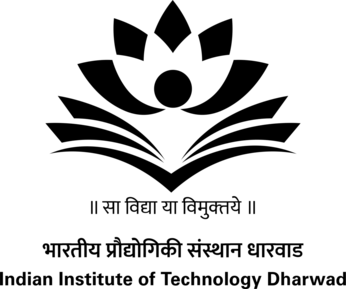
\includegraphics[width=4cm]{iitdhlogo}
			\end{figure}
		\end{block}
\end{columns}
\vfill
\begin{exampleblock}{Example Block}
The text goes here.. 
\end{exampleblock}
\end{frame}

\section[Tables]{Dynamic display of tables}
\begin{frame}{Dynamic Horizontal display (\texttt{$\backslash$pause\textless n-\textgreater})}
\begin{tabular}{lcccc}
  Class & A & B & C & D \\\hline
  X     & 1 & 2 & 3 & 4 \pause\\
  Y     & 3 & 4 & 5 & 6 \pause\\
  Z     &5&6&7&8
\end{tabular}
\end{frame}

\begin{frame}{Dynamic Vertical display (\texttt{$\backslash$onslide\textless n-\textgreater})}
\begin{tabular}{lc<{\onslide<2->}c<{\onslide<3->}c<{\onslide<4->}c<{\onslide}}
Class & A & B & C & D \\
  X     & 1 & 2 & 3 & 4 \\
  Y     & 3 & 4 & 5 & 6 \\
  Z     &5&6&7&8
\end{tabular}
\end{frame}

\section[Transitions]{Slide Transitions}

\begin{frame}{\texttt{$\backslash$transdissolve}}
\transdissolve
\lipsum[1-1]
\end{frame}

\begin{frame}{\texttt{$\backslash$transblindshorizontal}}
\transblindshorizontal
\lipsum[2-2]
\end{frame}

\begin{frame}{\texttt{$\backslash$transblindsvertical}}
\transblindsvertical
\lipsum[3-3]
\end{frame}

\begin{frame}{\texttt{$\backslash$transboxin}}
\transboxin
\lipsum[4-4]
\end{frame}

\begin{frame}{\texttt{$\backslash$transboxout}}
\transboxout
\lipsum[5-5]
\end{frame}

\begin{frame}{\texttt{$\backslash$transduration}}
\transduration{2}
\lipsum[12-12]
\end{frame}

\begin{frame}{\texttt{$\backslash$transwipe}}
\transwipe
\lipsum[11-11]
\end{frame}

\section[Maths]{Equations}

\begin{frame}{Multiline Equation}
\begin{eqnarray}
2x^2 + 3(x-1)(x-2)&=&2x^2 + 3(x^2-3x+2)\\
\pause &=& 2x^2 + 3x^2 - 9x + 6\\
\pause &=& 5x^2 - 9x + 6
\end{eqnarray}    
\end{frame}

\section{Plots}
\frame{
\frametitle{Incremental bar plot}
\setlength{\unitlength}{1 cm}

\begin{picture}(5,5)
  \linethickness{1 pt}
\put(0,0){\line(1,0){8}}%1.koord%
  \put(0,0){\line(0,1){5}}%1.koord%
\pause

%Jahr 98
\put(0.5,0){\line(0,1){2.3}}
\put(1,0) {\line(0,1){2.3}}
\put(0.5,2.3){\line(1,0){0.5}}
\put(0.5,-0.5){'98}
\invisible<1,3-10>{\put(0.5,2.5){17}} \pause
%Jahr 99
\put(1.5,0){\line(0,1){3.6}}
\put(2,0){\line(0,1){3.6}}
\put(1.5,3.6){\line(1,0){0.5}}
\put(1.5,-0.5){'99}
\invisible<1,2,4-10>{\put(1.5,4){27}} \pause
%Jahr 2000
\put(2.5,0){\line(0,1){4}}
\put(3,0){\line(0,1){4}}
\put(2.5,4){\line(1,0){0.5}}
\put(2.5,-0.5){'00}
\invisible<1-3,5-10>{\put(2.5,4.5){30}}\pause
%Jahr 2001
\put(3.5,0){\line(0,1){4.3}}
\put(4,0) {\line(0,1){4.3}}
\put(3.5,4.3){\line(1,0){0.5}}
\put(3.5,-0.5){'01}
\invisible<1-4,6-10>{\put(3.5,4.8){32}} \pause
%Jahr 2002
\put(4.5,0){\line(0,1){4.1}}
\put(5,0){\line(0,1){4.1}}
\put(4.5,4.1){\line(1,0){0.5}}
\put(4.5,-0.5){'02}
\invisible<1-5,7-10>{\put(4.5,4.6){31}} \pause
%Jahr 2003
\put(5.5,0){\line(0,1){4.1}}
\put(6,0){\line(0,1){4.1}}
\put(5.5,4.1){\line(1,0){0.5}}
\put(5.5,-0.5){'03}
\invisible<1-6,8-10>{\put(5.5,4.6){31}} \pause
%Jahr 2004
\put(6.5,0){\line(0,1){4.1}}
\put(7,0){\line(0,1){4.1}}
\put(6.5,4.1){\line(1,0){0.5}}
\put(6.5,-0.5){'04}
\invisible<1-7>{\put(6.5,4.6){31}}

\end{picture}
}

\section{Code}

\begin{frame}[fragile]{An Algorithm For Finding Primes Numbers.}
\begin{semiverbatim}
\uncover<1->{\alert<0>{int main (void)}}
\uncover<1->{\alert<0>{\{}}
\uncover<1->{\alert<1>{ \alert<4>{std::}vector<bool> is_prime (100, true);}}
\uncover<1->{\alert<1>{ for (int i = 2; i < 100; i++)}}
\uncover<2->{\alert<2>{ if (is_prime[i])}}
\uncover<2->{\alert<0>{ \{}}
\uncover<3->{\alert<3>{ \alert<4>{std::}cout << i << " ";}}
\uncover<3->{\alert<3>{ for (int j = i; j < 100;}}
\uncover<3->{\alert<3>{ is_prime [j] = false, j+=i);}}
\uncover<2->{\alert<0>{ \}}}
\uncover<1->{\alert<0>{ return 0;}}
\uncover<1->{\alert<0>{\}}}
\end{semiverbatim}
\visible<4->{Note the use of \alert{\texttt{std::}}.}
\end{frame}

\end{document}